
\section{Discovery and Characterization of Young Stellar Populations}
\def\secname{youngstars}\label{sec:\secname}

\noindent{\it P. Hartigan and C. Johns-Krull} % (Writing team)

\subsection{Introduction}

All young stars exhibit some form of 
photometric variability, and these variations hold the key
to understanding the diverse physical processes present at starbirth
such as mass accretion events from circumstellar disks, presence of
warps in envelopes, creation of new knots in stellar jets,
evolution of stellar angular momenta, starspot longevity and cycles, 
and the frequency and strength of flares. 
With the proper cadences and filter choices,
LSST will make a significant impact in our understanding of all
these phenomena simply by providing large enough samples to allow
us to relate these aspects of the young stars and their environments
to stellar properties such as mass, age, binarity,
and their location within their nascent dark clouds in a statistically
significant manner.

Low-mass ($\lessim 1.5 M_{\odot}$) pre-main-sequence stars divide
into two main categories, depending upon whether or not an optically thick
dusty circumstellar disk exists in the system: young stars without dusty
inner disks are known as `weak-lined T Tauri stars' (wTTs), while those
that have inner dusty disks are called `classical T Tauri stars'. Variability
behavior differs between wTTs and cTTs. The wTTs variability is dominated by
small-amplitude (typically $\sim$ 0.1 mag) quasi-periodic variations that arise
from cool star spots, though the active regions that generate X-rays in
these objects undoubtedly produce flares as well. Additional variations occur
among cTTs, primarily caused by unsteady mass infall from circumstellar disks
onto their stars, and from periodic extinction events that unfold as dense
clumps or disk warps circle the star in Keplerian orbits. 
At the extreme end of cTTs phenomena, rare
massive outbursts of several magnitudes with decay times between several months
to over a hundred years in pre-main-sequence stars (EX Ori's and FU Ori's)
are of great interest to studies of disk accretion because they indicate the onset of
a major instability. Only a handful of such systems have been found, and LSST
will easily detect them along with similar, less-dramatic systems.

Obtaining rotation periods for large numbers of pre-main-sequence stars is the only way to
quantify how the angular momenta of young stars vary with age. For both wTTs and cTTs,
phase-coherence in the rotation periods defines the longevity of star spots, while the 
amplitude of the periodic component of the lightcurve constrains the spot coverage (and
temperature if multiple filters are used). In cTTs, U-band fluxes rise during
accretion events, which we can distinguish from extinction events if red magnitudes are
also available. A large accretion event is a signal to observe the system
in the future with other instrumentation to look for evidence of a newly-created
jet knot. Flaring activity is easiest to monitor at U, though the rapid decline of
flares requires a rapid cadence to capture correctly.

LSST also provides a potential means to discover new young stars by way of
their variability and colors. One of the challenges in this regard will be to
distinguish young stars from other low-amplitude variable stars in the field.
In that regard we expect that machine-learning techniques that incorporate knowledge of
fluxes in other wavebands as well as the LSST lightcurves and colors will
be an ongoing effort. It is possible that X-ray detections will be more
reliable for detection of new young stars, but LSST will at minimum assist
by identifying non-YSO X-ray sources, and should be a means for discovery
for older pre-main-sequence stars (10 $-$ 30 My range) that have had time
to wander away from the well-known sites of star forming activity that are
typical targets for deep, pointed X-ray surveys

% --------------------------------------------------------------------

\subsection{OpSim Analysis}
\label{sec:\secname:analysis}

{\bf Target Regions}

Young stars congregate in specific regions, so it is worthwhile to
consider which of these areas will be the most fertile for studies with LSST.  
The closest star forming regions are all about 140~pc distant: Taurus-Auriga in
the north and $\rho$ Oph, Lupus, Cha I, and CrA in the south. However,
these regions have only low-mass molecular clouds, and each contain
only about 100 young stars. More massive molecular clouds produce both higher
mass stars and more low mass stars. In Orion (d = 414 pc), the number of
identified YSOs is $\sim$ 3000, and we expect $\gtrsim$ 30000 pre-main-sequence
stars in the famous southern star formation region in Carina (2.3 kpc).
LSST will make its greatest impact
when observing the more massive star formation regions, where the amount
of young stars is much higher.

Owing to extinction in the dark clouds,
source confusion will generally not be an issue (as evidenced by typical
deep optical images of such regions), though the large fraction
of pre-main-sequence binaries at all separations ensures that many
lightcurves will be composites of the primaries and secondaries. 
More distant star-forming regions will suffer from enhanced foreground 
contamination, though it should be possible to eliminate most contaminating
variable stars by combining close inspection of their lightcurves with
colors.

{\bf Metrics:}

{\bf A. Magnitude Limits, Filter Choices}

To quantify YSO studies with LSST, we consider V~927 Tau, 
a rather faint, moderately-reddened 0.2 M$_\odot$ young star in the Taurus cloud
as a target goal. Extrapolating this star
to the distance of Carina we have u=24.0, g=23.0, r=20.8, i=19.4, and z=18.0. For reference,
a typical young star in the Carina X-ray catalog has an i-magnitude of 18.
Objects that suffer larger extinctions along the line of sight will
be easiest to observe in the red. The universal cadence option of 2$\times$15 sec
exposures will yield $\sigma$ = 0.02 mag for r=21.8, a magnitude fainter than
V~927 Tau would be in Carina. We show below that this photometric uncertainty 
suffices to recover a typical period from such an object. The mass function
of young stars appears to peak around 0.3 M$_\odot$, so LSST will 
determine periods below this mass peak with nominal r-band measurements
for a region like Carina. Of course, several additional magnitudes of extinction will
exist towards many embedded sources. For example, if we assume an additional five magnitudes
of extinction at V for the V~927 Tau-like example above,
then r=25.2 and $\sigma$ = 0.41 mag per visit with universal cadence,
so no usable lightcurve will be possible at r. 
However, z=20.5 in this case, where $\sigma$ $<$ 0.01 mag and precision
lightcurves are again possible. 

{\bf B. Period Recovery for wTTs}

In order to assess how well LSST will recover periods, we created the following
model for wTTs variability.  Based on current surveys of wTTs, the periods are
distributed approximately as a Poisson distribution with a mean of 3.5 days
\citep[Affer et al. (2013)]{Affer13}. 
Amplitudes are typically 0.1 magnitude \citep[(Grankin et al. 2008)]{ROTOR},
, so we adopt a Poisson distribution 
that has a mean amplitude of 0.05 mag, and then add 0.05 mag to ensure that
the mean variability is 0.1 mag. Shapes of T-Tauri lightcurves can be sinusoidal,
but many are `bowl-shaped', influenced by the distribution of large dark starspots
\citep[(Alencar et al. 2010)]{CoRoT}.
For the bowl lightcurves we assumed a Gaussian shape with a FWHM in a uniform
distribution of extent between 0 and 0.75 in phase.
Our simulations cover both of these shapes.
Errors for each point were taken to be 0.02 magnitude, corresponding to
about r $\sim$ 21.8 for a universal cadence. 

One set of simulations assumed a cadence of
one observation every three days over the course of a year.
If we define a successful period recovery to be better than a 1\%\ error, then
using the standard Scargle method \citep[(Horne \& Baliunas 1986)]{Scargle}
we are able to find the correct period in
98\%\ of the the sinusoidal, and 86\%\ of the bowl lightcurves, with the most
difficult challenges being at the short end of the period distribution. If we change
the cadence to once every 7 days, the ability to recover periods drops to
82\%\ and 59\% , respectively, for the two shapes. Interestingly, restricting the
sample to the highest-amplitude sources ($\gtrsim$ 0.1 magnitude) does little
to aid period recovery. The main issue remains the short-period systems where
P $\lesssim$ 2 days. 

\begin{figure}[b]
\begin{center}
 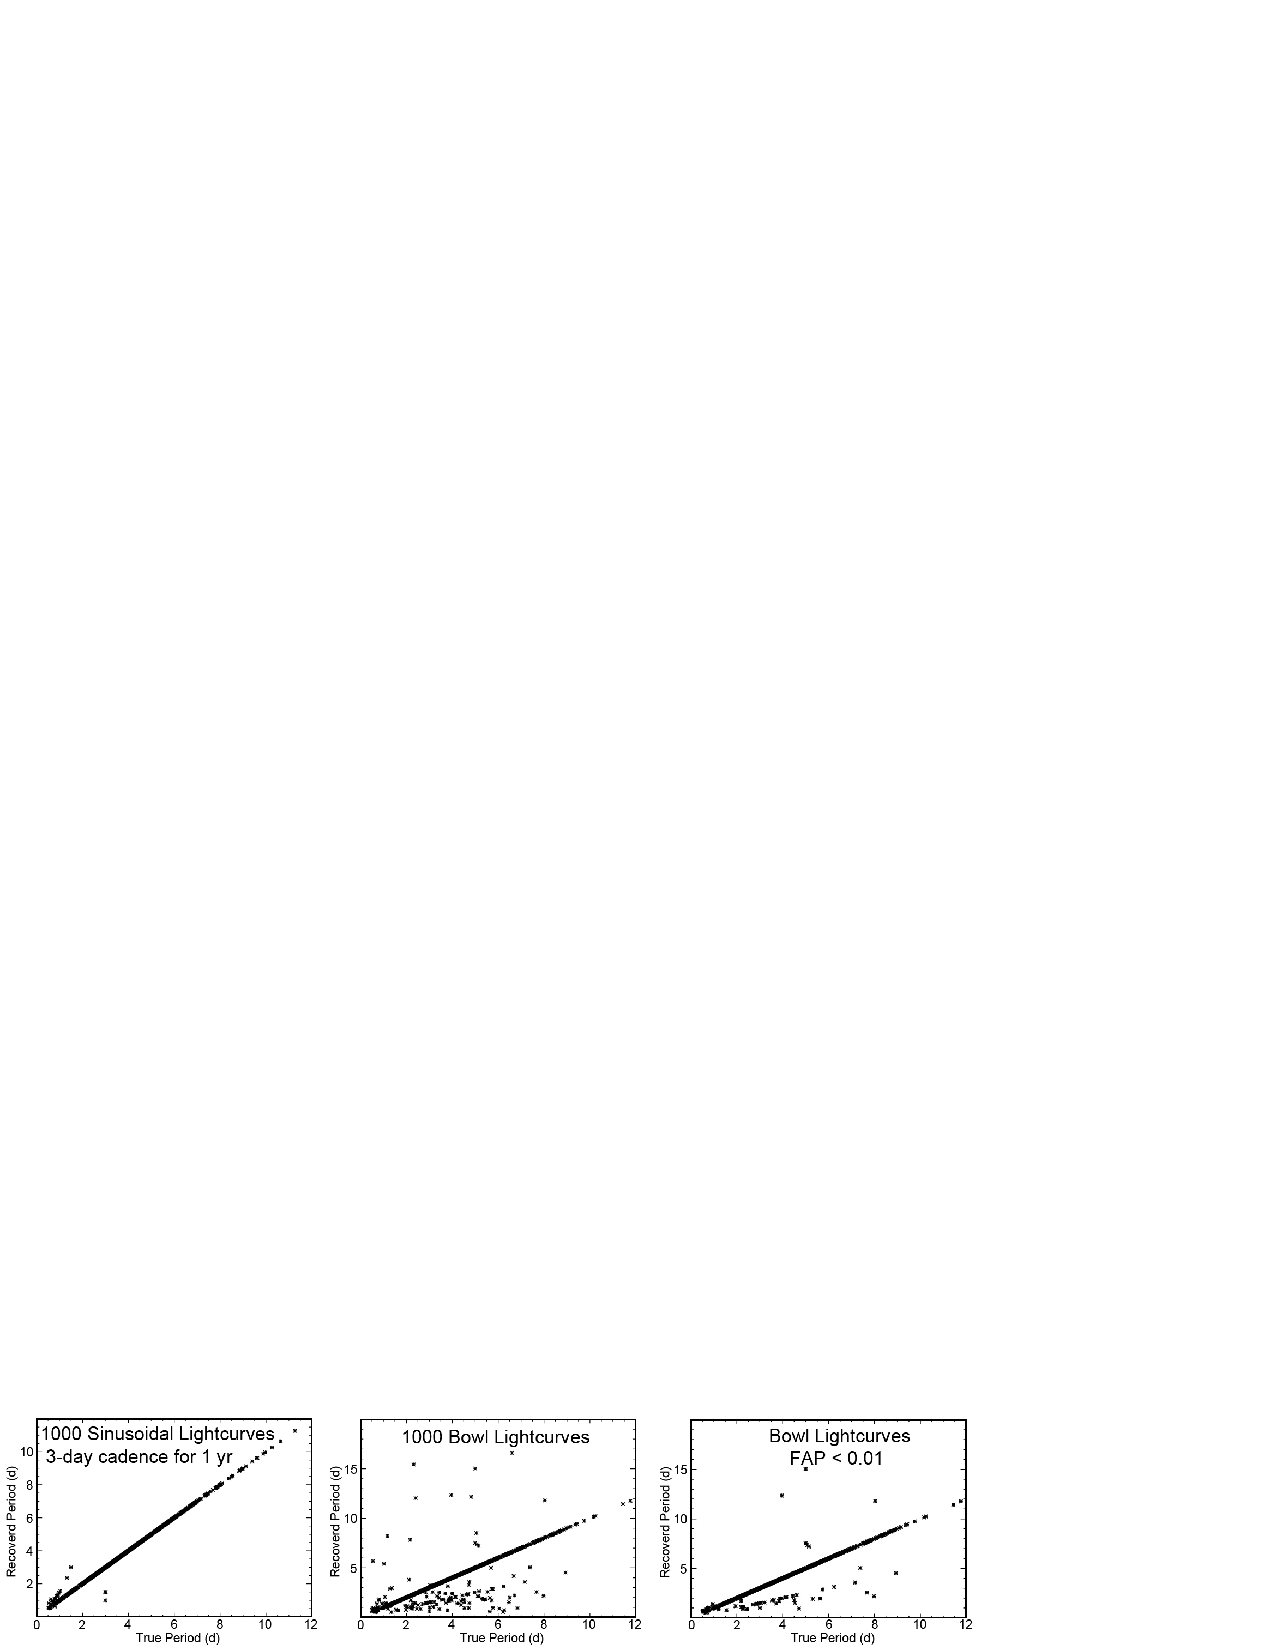
\includegraphics[width=5.32in]{figs/starFormation/tts1.pdf}
 \caption{Recovered period vs. true period for a sample of sinusoidal (left),
bowl-shaped (middle) and bowl-shaped with False Alarm Probability $<$ 0.01 (right),
assuming a 3-day cadence and one year of observing. What appears as a solid line are the
individual points with periods that are recovered correctly. The bowl-shaped curves are
more difficult to recover than the sinusoids, but the method is highly successful in both cases.}
   \label{tts1}
\end{center}
\end{figure}

\begin{figure}[b]
\vspace*{1.0 cm}
\begin{center}
 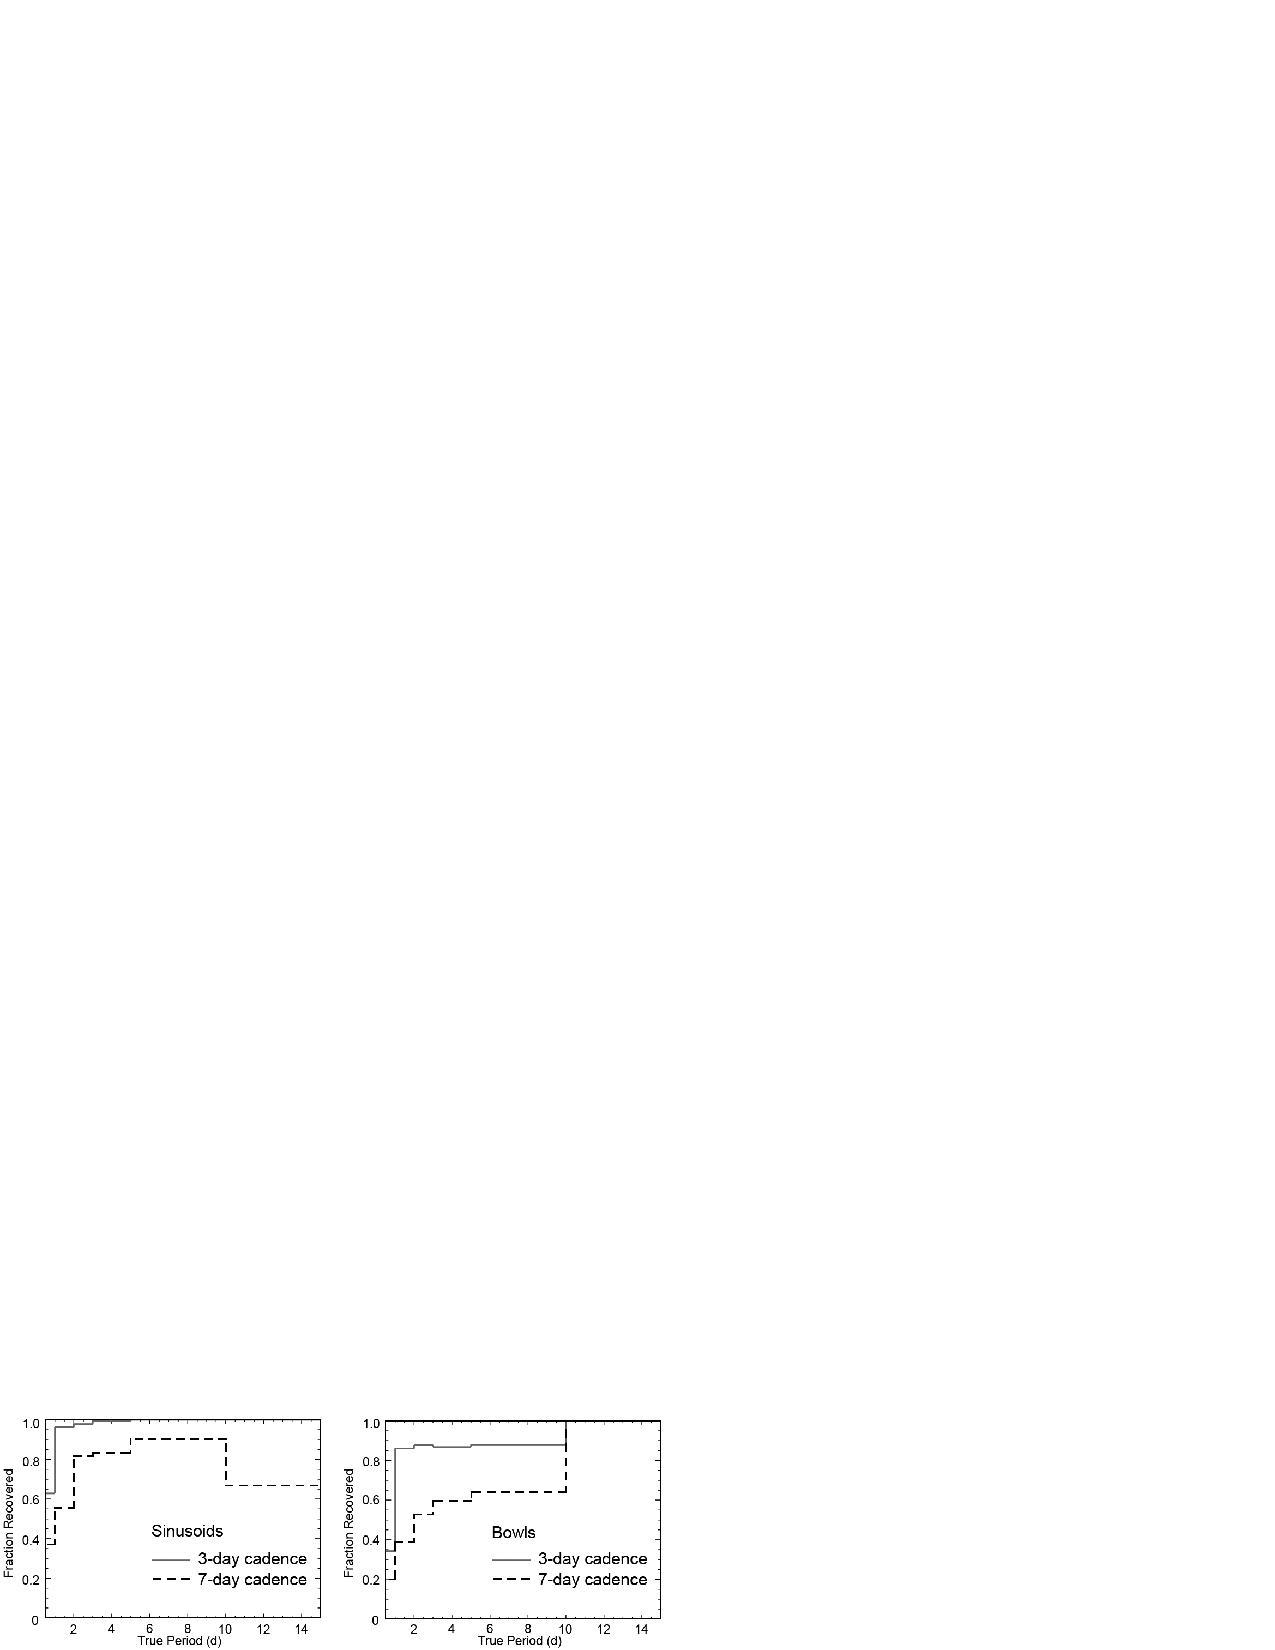
\includegraphics[width=5.32in]{figs/starFormation/tts2.pdf}
 \caption{ Fraction of periods recovered correctly for sinusoidal (left) and bowl light curves (right) for
3-day (solid line) and 7-day (dashed line) cadences over an observing period of one year.
A 3-day cadence is significantly better than a 7-day one. Over 98\%\ of sinusoidal, and 86\%\ of bowl
light curve periods are recovered successfully with the 3-day cadence. The percentages drop to about
82\%\ and 59\%\, respectively, for the 7-day cadence.
}
   \label{tts2}
\end{center}
\end{figure}

\begin{figure}[b]
\vspace*{1.0 cm}
\begin{center}
 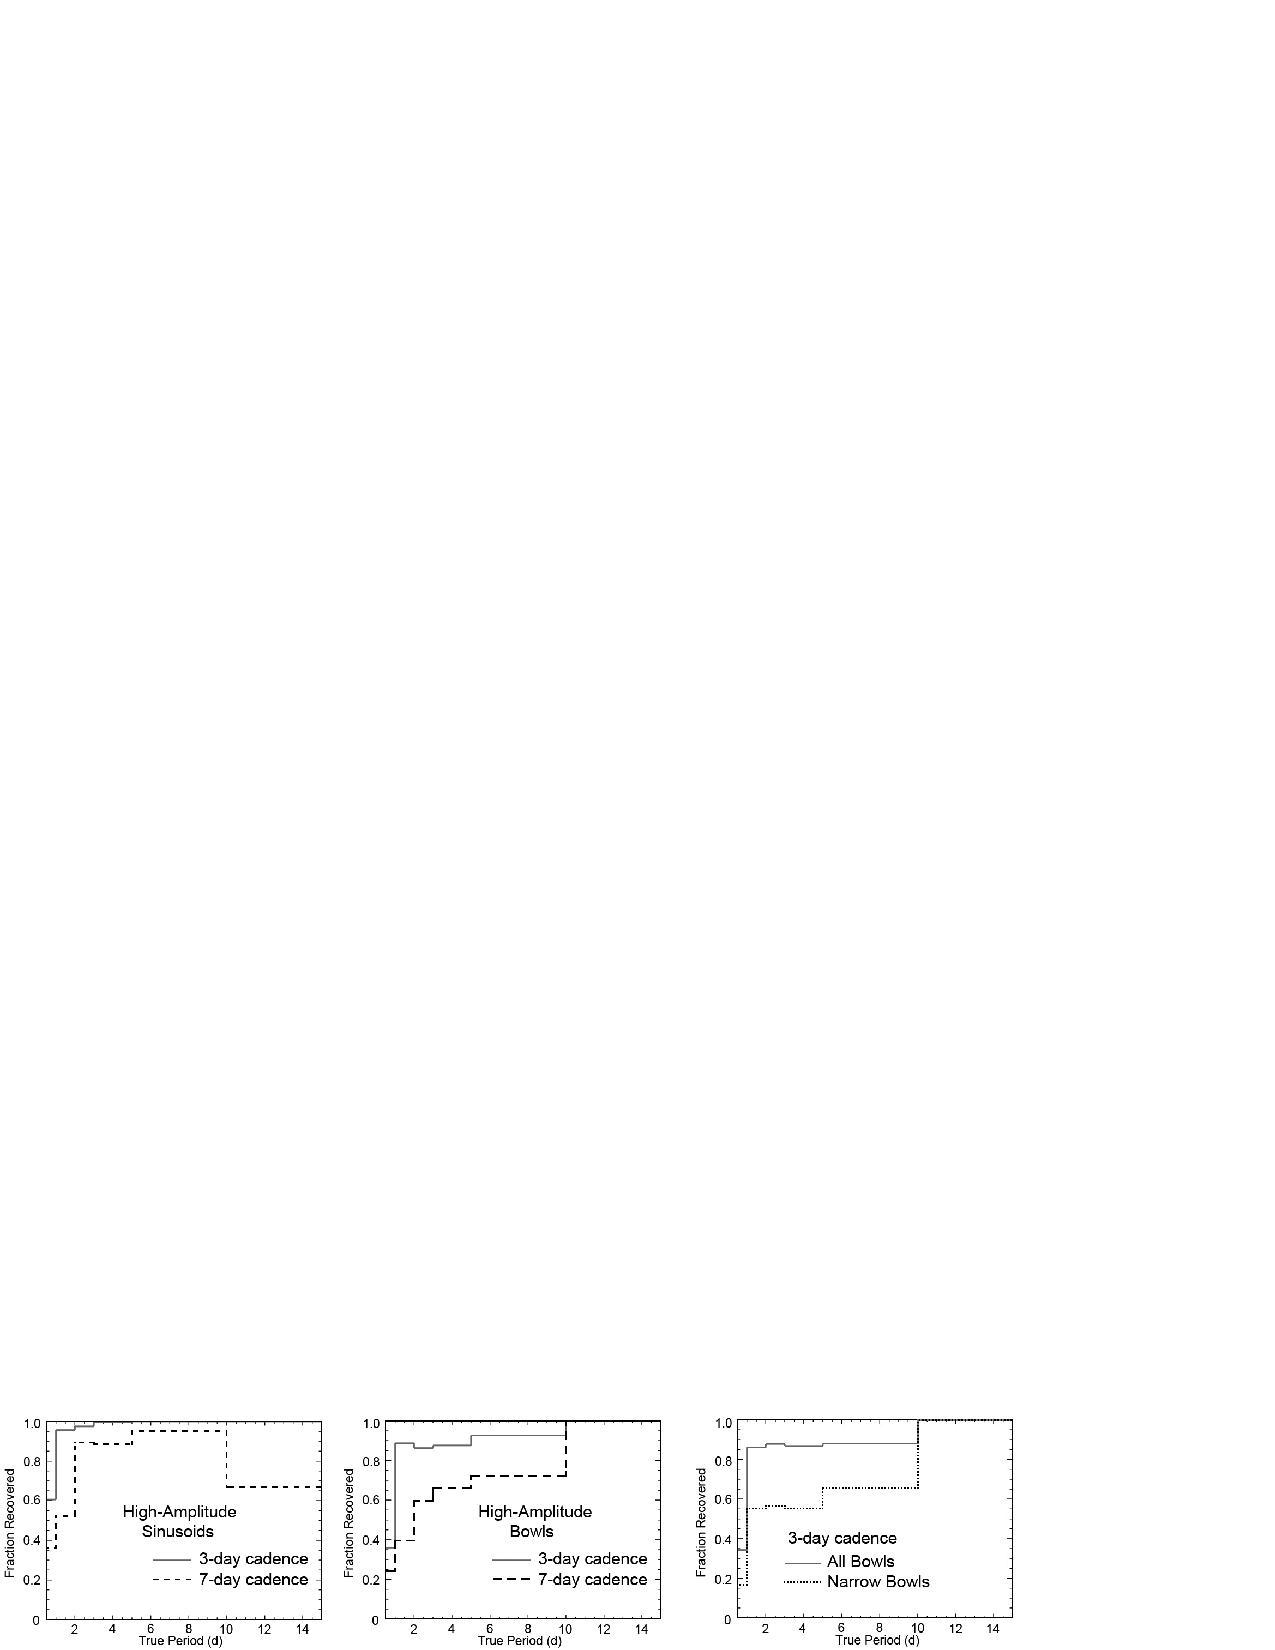
\includegraphics[width=5.32in]{figs/starFormation/tts3.pdf}
 \caption{Left and center: Same as Fig 2 but restricting the sample to amplitudes greater than 0.1 mag. The
method is only marginally more successful with the larger amplitude objects than it is with the entire sample.
Right: The narrowest 278 bowls have a significantly higher error rate than the entire sample does.
}
   \label{tts3}
\end{center}
\end{figure}

Overall, standard cadences of once every few days should suffice
to find most periodic T-Tauri stars that have periods $\gtrsim$ 3 days. 
A dedicated campaign to observe star-forming regions 
at time intervals of an hour or less is required to capture the shorter-period systems.
The r-filter should suffice for most objects, though some benefit will be had
by going to z to allow the more heavily-extincted sources to be observed.

{\bf C. Period Recovery for cTTs}

Complex irregular variations in cTTs lightcurves make it much more difficult,
and in many cases impossible to
recover periods in these systems. While sparse coverage of one observation every
few days is adequate for identifying sudden changes from accretion events, these
events to a large degree overwhelm low-amplitude periodic signatures. Even when
period searches yield a low false-alarm probability, the results are not necessarily
reliable. Results from Palomar Transient Factory surveys in the North American
Nebula \citep[(Findeisen et al. 2013)]{feindeisen13} and with Spitzer
\citep[(Cody et al. 2014)]{cody14} 
reveal several types of both short- and long-term variations including both bursting and
fading.  These observations emphasize how important it will be to have some
dense phase coverage as a reality check to ensure the reliability of
any periods recovered from sparse data in these objects, as well as to
follow the short-term variations that characterize accreting systems.

{\bf D. Discovery, Accretion and Extinction Events}

As we indicated above, any
cadence will uncover FU Ori and EX Ori events in all filters.
Periodic extinction events follow the same restrictions and
have the same requirements as rotational periods described in subsection B.


% --------------------------------------------------------------------

\subsection{Summary and Recommendations}
\label{sec:\secname:discussion}

{\bf Performance for Nominal Cadences}

Nominal cadences that return to a star-forming region every 3-4 days
will suffice to determine rotation periods for $\sim$ 90\%\ of the 
young stars within the magnitude limits of LSST. 
These cadences are also adequate to detect major episodic
accretion events like FU Ori's and EX Ori's.

{\bf The Need for Annual Dense Coverage of a Few Selected Regions}

Occasional dense coverage of targeted regions is the only way to
get quantitative information on short-term accretion and flare
activity.  Dense coverage also removes degeneracies
for periodic variables that have periods less than a day, and is
the only way to provide a sanity check on any periods recovered for
cTTs, which have complex irregular light variations.
Comparing longevities of starspots across the mass ranges of young
stars requires two well-sampled lightcurves separated by large
time intervals. 

These goals can be accomplished by having a week every year where
one or more selected fields are observed once every 30 minutes in u, r and z.
A young star with a 2-day period sampled every 30 minutes provides a 
data point every 0.01 in phase. For the best-case scenario, observing for 7 nights
and 10 hours per night would yield 140 photometric points in each filter.
Depending on the period aliasing, this coverage should populate the
phases well enough to identify most of the large starspots on the stellar photospheres.

At the beginning of LSST operations we argue that three targeted test fields
be observed in this manner to illustrate what can be done with LSST in this mode.
Combining a densely-packed short-interval
dataset with a sparse but long baseline study maxmizes the scientific return
for both methods, and allows LSST to address all of the phenomena
discussed in the Introduction.

% ====================================================================

% bibtems need pushing into the relevant file!

%\bibitem[Affer et al. (2013)]{Affer13}
%{Affer, L., Micela, G., Favata, F., Flaccomio, E., \& Bouvier, J.} 2013
%\textit{MNRAS}, 430, 1433

%\bibitem[Alencar al. (2010)]{CoRoT}
%{Alencar, S. H. P. et al.} 2010,
%\textit{A\&A}, 519, A88

%\bibitem[Cody al. (2014)]{cody14}
%Cody, A., et al.
%{Cody, A. et al.} 2014,
%\textit{AJ}, 147, 82 

%\bibitem[Grankin al. (2008)]{ROTOR}
%\bibitem[Findeisen al. (2013)]{findeisen13}
%Findeisen, K., Hillenbrand, L., Ofek, E., Levitan, D., Sesar, B., Laher, R., \& Surace, J.
%{Findeisen, K. et al.} 2013,
%\textit{ApJ}, 768, 93 

%\bibitem[Grankin al. (2008)]{ROTOR}
%{Grankin, K. N., Bouvier, J., Herbst, W., \& Melnikov, S. Yu.} 2008,
%\textit{A\&A}, 479, 827

%\bibitem[Horne \& Baliunas (1986)]{Scargle}
%{Horne, J. H. \& Baliunas, S.} 1986, \textit{ApJ}, 302, 757

\navigationbar
